\chapter{Implementation, results and discussion}
\label{chap:Method}
This chapter begins with a detailed exploration of the processes and methodologies employed to implement GNNs for the predictive analysis of nozzle flows. In the subsequent section, we introduce the Graph U-Net architecture, outline its implementation settings, present the results obtained, and validate them with the simulation outcomes. This discussion sets the stage for the development of three modified surrogate models with the aim of enhancing model performance, detailed in Section \ref{proparch}. Through quantitative analysis and performance evaluation, we identify the successes and challenges encountered in modelling nozzle flow dynamics with GNNs. Thus, this chapter demonstrates the practical implementation of the proposed methodologies and performs a critical examination of the results and the efficacy of these models.
\section{Data pre-processing} \label{prep}
In this section, we describe the process for dataset preparation, how the data from CFD simulations are extracted and converted into graph-structured formats that facilitate efficient GNN training. It includes dataset generation from nozzle flow simulations at varied conditions, transformation of unstructured mesh data into a graph format for GNN compatibility, and the specification of GNN inputs and outputs. 
\subsection{Dataset generation}
Nozzle simulations are carried out for 120 cases, each with a different set of Inlet 1 and Inlet 2 velocities. The velocity ratio between the two velocities lies in the range of [1, 10]. Velocity ratio in our case refers to the ratio of higher velocity to lower velocity.
%  such that the velocity ratios between the inlets range from 1 to 9.  (Velocity ratio in our case refers to the ratio of higher velocity to that of lower velocity) 
% The simulation results, i.e; the steady-state fields are logged after 1000 and 30000 time-steps. The \gls{CFD} results at 1000 time-steps are still developing and are unstable whereas those at 30000 steps are observed to be stable solutions. Hence, the simulation results after 30000 steps are taken as the ground truth values or target data, while the input to the surrogate model are the results after 1000 steps. The input and target datasets are then transformed into graph data, normalized, and passed to the network. 
Simulation data are obtained at two intervals: after 1000 and 30000 iterations or steps. The results at 1000 iterations, which are still developing and unstable, serve as inputs to the surrogate model. Whereas, the results at 30000 iterations, which represent stable solutions, are considered the ground truth or target data for model training. These results are then transformed into graph data, which encapsulate the spatial relationships and properties of flow fields. The GNN architecture is designed to learn these features and predict stable, steady-state fields from the early, unstable simulation results.
\subsection{Transformation of mesh data to graph data}
Conventional RANS solvers require substantial distances from domain boundaries to mitigate adverse effects on solutions around the region of interest. However, this is not required for the deep learning task. Hence, we narrow our attention to a small region just enclosing the nozzle, as seen in Figure \ref{clipmesh}. We clip the CFD mesh appropriately and resample the velocity and pressure fields to this mesh with reduced spatial extent. We define the cell centers on the clipped mesh and assign them as the nodes of the graph. Two adjacent cells $i$ and $j$ (cells that share an edge) in this resulting unstructured mesh are represented as nodes $v_i$ and $v_j$ on the graph and are connected by an edge $e_{ij}$. The graph connectivity is then given by the edge index data structure, which comprises two lists - one stores the source node indices, and the other has the destination node indices. CFD solvers typically assign pressure, velocity and other fields to each cell of the mesh, whereas graphs require node features, i.e.; fields defined on each node. Therefore, the cell data (fields) are converted to point data at the cell centers, making them suitable for graph representation. The simulation data is then saved in a \verb|hdf5| format. This is then directly used to read pressure, velocity and co-ordinate information at cell centers. 
% $u_{x}$, $u_{y}$, $p$, $c_x$, $c_y$, and $\gamma_{\operatorname{tag}}$. 
The edge index data required for the GNN is generated by computing adjacent cells and storing their indices in a \gls{COO} format. 
\begin{figure}[ht]
    \centering
    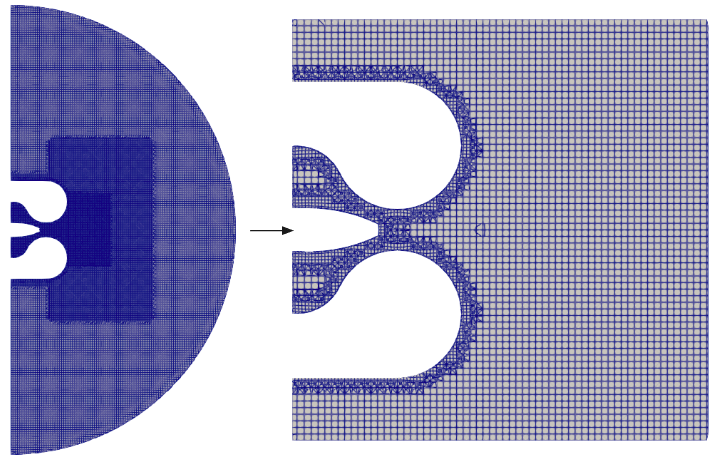
\includegraphics[width=10cm]{images/Methodology/Clipped.png}
    \caption{Depiction of the area of focus - the original CFD mesh (left) is clipped and transformed into the region of interest (right)}
    \label{clipmesh}
\end{figure}
\begin{figure}[ht]
    \centering
    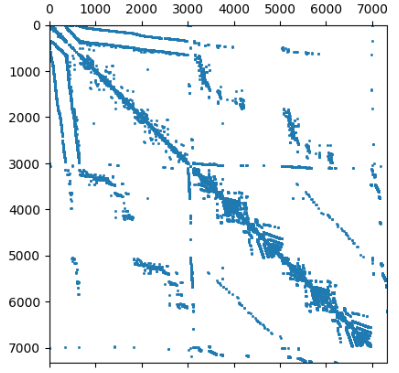
\includegraphics[width=6cm]{images/Methodology/AdjMatrix.png}
    \caption{Visualization of the adjacency matrix representing the graph connectivity of the clipped, unstructured mesh with 7329 nodes.}
    \label{adjmat}
\end{figure}
\subsection{Model inputs and outputs}
After data pre-processing, the simulation mesh is considered as a bidirectional graph $G = (V, E)$ where the set of \gls{N} nodes denoted as $V$ are linked by the set of edges $E$ of the graph. To construct a graph, we need,
\begin{itemize}
\item A feature description, consolidated into an $N \times D$ feature matrix $X$, where \gls{D} denotes the number of input node features.
\item The graph connectivity or relationships within nodes is represented in matrix form as an adjacency matrix, $A$ or as an edge set $E$ of the shape $2 \times P$, where $P$ is the number of pairs of connected nodes in $E$.
\end{itemize}
Let each node have \gls{fx} features, and \gls{fy} predictions. The GNN maps the set of node features and edge index matrices to predictions as, 
\begin{equation}
    \mathrm{GNN}: \mathbb{R}^{{N} \times F_{\mathrm{X}}}, \mathbb{W}^{2 \times P} \rightarrow \mathbb{R}^{{N} \times F_{\mathrm{Y}}}
    \end{equation}
We then get a graph-level output of the shape ${N} \times F_{\mathrm{Y}}$. The node feature vector $\mathbf{x}_i$ and prediction vector $\mathbf{y}_i$ of interest at each node $v_i$ is given as,
\begin{equation}
    \begin{aligned}
    & \mathbf{x}_i=\left[u_{x, i}, u_{y, i},c_{x, i}, c_{y, i}, \gamma_{\operatorname{tag}, i}\right] \\
    & \mathbf{y}_i=\left[u_{x, i}, u_{y, i}, p_i\right]
    \end{aligned}
\end{equation}
where $u_{x, i}$ and $u_{y, i}$ are the node velocities in X and Y directions, $p_i$ is the node pressure, and \gls{cxi} and \gls{cyi} are the spatial co-ordinates of the nodes. \gls{gammatag} is the node tag that defines which cell the node belongs to: inlet, walls or internal mesh. To summarize, our model has 5 input channels (representing node features) and 3 output channels (denoting node predictions). In addition to these channels, the GNN model also requires an edge index matrix to internally compute the adjacency matrix for the graph. 
\subsection{Data normalization}
Data normalization is performed on both input channels (node features) and output channels (target vectors), carried out using the three steps outlined below.
\begin{enumerate}
\item Following common practice, we normalize all the fields of interest with respect to the magnitude of free-stream or reference velocity $u_0$ to make them dimensionless. 
\begin{equation}
    \Tilde{u}=u /\left\|u_0\right\|, \quad \Tilde{p}=p /\left\|u_0\right\|^2
\end{equation}
The latter plays a crucial role as it eliminates the quadratic scaling effect present in the pressure values of the target data, effectively flattening the solution space, thereby simplifying the task for the neural network in subsequent stages.
\item Next, we subtract the mean pressure from the dimensionless pressure values. 
\begin{equation}
\hat{p} = \Tilde{p} - p_{mean} , \quad \text{where} \quad p_{mean} = \sum_i p_i / n
\end{equation}
$n$ is the number of training samples and $p_i$ denotes individual pressure values. Without this step, the pressure targets depict an ill-posed learning objective since the random pressure offsets in the solutions lack correlation with the inputs.
\item As a final step, every channel undergoes normalization to the range of [-1, 1] or [0,1]. This standardization aims to mitigate errors stemming from finite numerical precision during the training period. We opt for the maximum absolute value of each quantity across the entire training dataset to normalize the data. 
\end{enumerate}
After performing normalization, we shuffle the entire dataset, split it into 3 parts and distribute it as training data, validation data and test data in the ratio of 80:10:10. 
\section{Graph U-Net}
Here, we introduce the Graph U-Net architecture, a foundational framework for the surrogate models used in this work. We analyze the benefits and shortcomings of this model as well as explain the motivation behind developing a modified GNN.
% Some important aspects of graph convolutions are detailed below. 
% \begin{enumerate}
% \item \textbf{Aggregation of neighbor information:} Each node aggregates the features of its neighbors, weighted by the parameters learned in the weight matrix $W^{(l)}$. This process enables nodes to incorporate information from their local neighborhoods, capturing relational dependencies and structural patterns in the graph. 

% % The normalization factor $c_{ij}$ ensures that the aggregated features are appropriately scaled based on the connectivity of nodes.
% \item \textbf{Weight sharing:}
% The weight matrix $W^{(l)}$ is shared across all nodes, allowing the model to capture common patterns and relationships present in the graph. By sharing parameters, GCNs can effectively learn representations from limited labeled data, facilitating transfer learning and adaptation to new graphs or domains.
% \item \textbf{Hierarchical feature learning:}
% GCNConv layer enables hierarchical feature learning by iteratively aggregating information from neighboring nodes. As information propagates through multiple layers, nodes can capture increasingly abstract and high-level features of the graph. 
% \end{enumerate}
\subsection{Architecture}
The downsampling operation is carried out using the top-k pooling strategy, which retains the most important nodes in the graph while discarding less relevant nodes based on a specified criterion. GCNConv layers are used as the convolutional layers in Graph U-Nets. Here, unpooling is not a distinct operation like in traditional U-Nets. Instead, skip connections are used to implicitly perform unpooling. During decoding, downsampled features from the encoder are combined with zeros or empty features in the decoder using skip connections. This integration effectively restores spatial details and contextual information from the original input graph, ensuring that important features are retained and allowing for the recovery of detailed graph structures. Therefore, unpooling in Graph U-Net is seamlessly integrated into the skip connection mechanism, facilitating the reconstruction of the original graph resolution during decoding. Figure \ref{fig:GraphUnet} presents a schematic overview of the Graph U-Net architecture. 
\begin{figure}[ht]
    \centering
    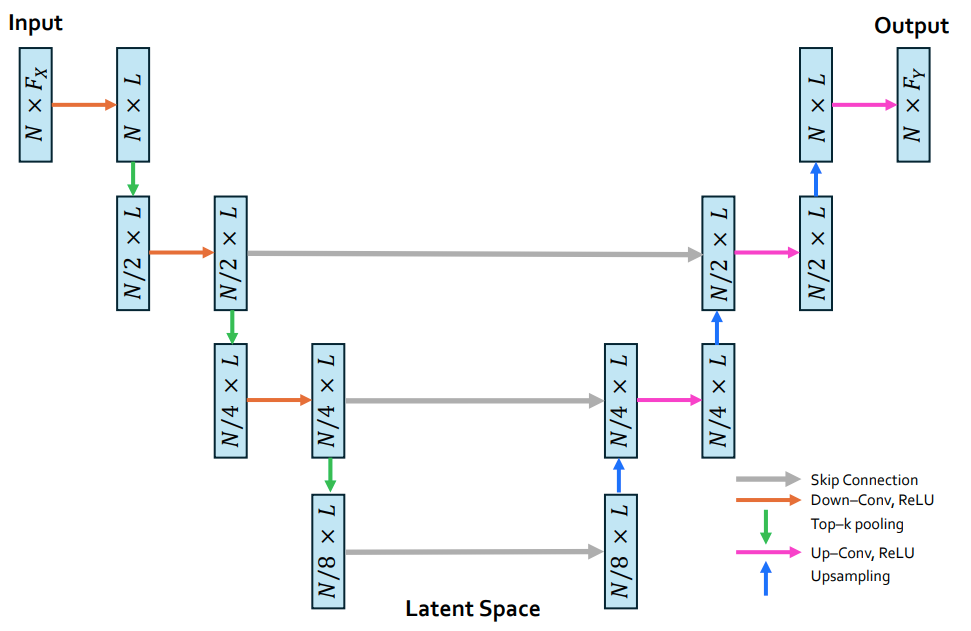
\includegraphics[width=12cm]{images/Methodology/GraphUNet.png}
    \caption{Detailed view of the Graph U-Net architecture applied to fluid dynamics, showcasing an encoder-decoder structure with skip connections. Each layer’s application is annotated with the resultant dimensions, illustrating the feature reduction or expansion throughout the network. Here, L is the number of channels in a convolutional layer.}
    % , N is the number of nodes in the graph, and F$_X$ and F$_Y$ denote the number of input and output features respectively.}
    \label{fig:GraphUnet}
\end{figure}
\subsection{Results and discussion}
We develop a surrogate model that uses the exact Graph U-Net architecture. As a first step, we are interested in investigating the ability of the model to reproduce the target data, i.e.; when the same target data is given as input. This means that the task solely performs reconstruction of the target dataset without requiring prediction. We also go on to perform the prediction task with the same model architecture, which forms the baseline for all the other architectures proposed in this work. The following settings are maintained for both the reconstruction and prediction tasks. We implement a 9-fold cross-validation for the training process. The initial learning rate is set to $0.0005$, and a Step LR scheduler is used to decay the learning rate by a factor of $0.75$ after every 100 epochs. We use the Adam optimizer and train on the RMSE loss for 500 epochs. The model's hyperparameters are selected by a hyperparameter tuning process. Table \ref{table:complex} presents the model complexity and performance on varying the number of channels and hidden layers. It is to be noted that each hidden layer refers to the combination of sampling (pooling and unpooling) and convolution operations (up and down convolutions). That is, if we perform the pooling and convolutions $d$ times in the encoder and reverse this process $d$ times in the decoder, the number of hidden layers in this architecture is taken as $d$. \\
\begin{table}[ht]
    \centering
    \caption{Hyperparameter tuning - Table depicting the number of channels, hidden layers, trainable parameters, training loss, and validation loss, measured with the RMSE criterion, for the Baseline architecture corresponding to each setting.}
    \label{table:complex}
    \begin{tabular}{|c|c|c|c|c|}
    \hline
    \textbf{Channels} & \textbf{Hidden layers} & \textbf{Trainable parameters} & \textbf{Training loss} & \textbf{Validation loss}\\
    \hline
    \multirow{4}{*}{48} & 2 & 7k &  0.04876&  0.05166\\
    \cline{2-5}
                        & 3 & 12k &  0.04713&  0.05128\\
    \cline{2-5}
                        & \textbf{4} & \textbf{17k} & \textbf{0.04386}&  \textbf{0.05237}\\
    \cline{2-5}
                        & 5 & 22k &  0.04272 &  0.05299\\
    \hline
    \multirow{4}{*}{64} & 2 & 13k & 0.04536&  0.05349\\
    \cline{2-5}
                        & 3 & 21k & 0.05074 &  0.05472\\
    \cline{2-5}
                        & 4 & 30k &  0.04139&  0.05615\\
    \cline{2-5}
                        & 5 & 31k & 0.04692 &  0.05587\\
    \hline
    \multirow{4}{*}{128} & 2 & 51k& 0.03983&  0.05639\\
    \cline{2-5}         
                         & 3 & 84k & 0.03840&  0.05492\\
    \cline{2-5}
                         & 4 & 117k & 0.03642 &  0.05341 \\
    \cline{2-5}
                         & 5 & 150k &  0.05011&  0.05563\\
    \hline
    \end{tabular}
    
    \end{table}
Out of the various architectures, we select the model that gives the lowest training loss and validation loss, or one that offers a good compromise between the two losses. Among the models with similar performance, we choose the one that is the simplest, i.e.; has relatively feweer trainable parameters, without compromising on accuracy or facing the risk of overfitting. Hence, we execute the training process using a GNN architecture with 48 channels and carry out the sampling and convolution operations 4 times (number of hidden layers) on the encoder and the decoder sides. Similar experiments have been conducted to choose the ideal batch size, activation function and other hyperparameters. The key hyperparameters are listed in Table \ref{table:hp}. 
\begin{table}[ht]
    \centering
    \caption{Model hyperparameters}
    \label{table:hp}
    \begin{tabular}{|l|l|}
    \hline
    \textbf{Hyperparameter}    & \textbf{Value/Description} \\
    \hline
    Channels    & 48                           \\
    \hline
    Hidden layers    & 4                          \\
    \hline
    Pooling ratios             & [0.5,0.5,0.5,0.5]                       \\
    \hline
    Batch size                 & 4                         \\
    \hline
    Activation function        & ReLU                       \\
    \hline
    Weight initialization    &  Kaiming                        \\
    \hline
    Initial learning rate       & 0.0005                       \\
    \hline
    \end{tabular}
    \end{table}
\subsubsection{Reconstruction task}
As mentioned previously, we prescribe the same steady-state CFD dataset as the input and target data to evaluate the effectiveness of reconstruction of the Graph U-Net model. The CFD results, predictions of the GNN model and the absolute difference between them for four simulation cases from the test dataset are shown in Figure \ref{blrecon}.\\
\begin{figure}[ht]
    \centering
    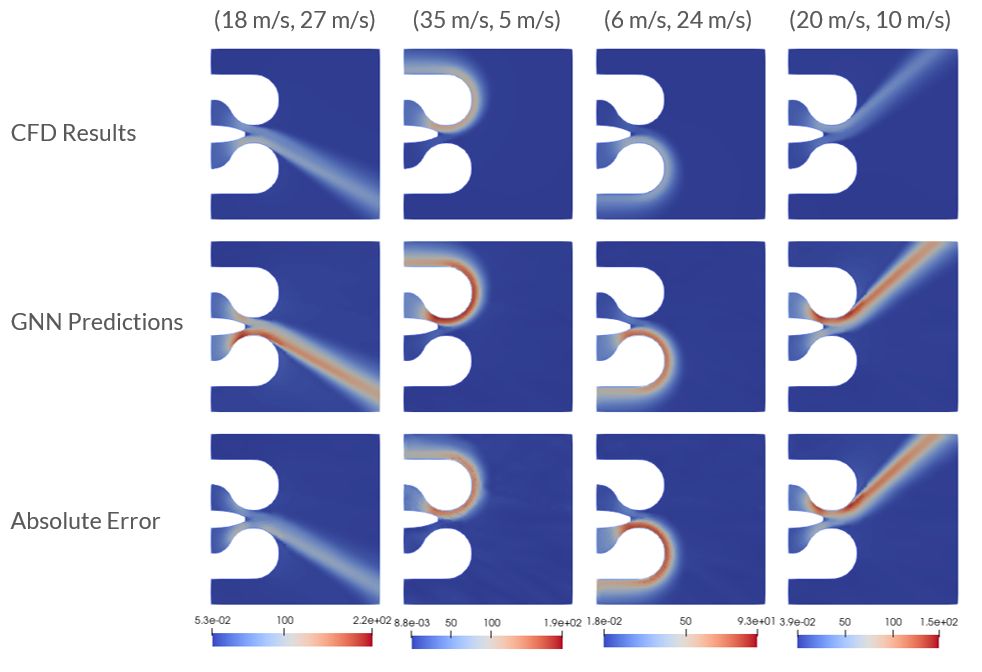
\includegraphics[width=14cm]{images/Methodology/allvelrecon.png}
    \caption{Visualization of velocity fields for four cases from the baseline's reconstruction task, with inlet velocity values prescribed as (Inlet 1, Inlet 2). Here, the first row represents the target data, the second row corresponds to the model predictions, and the last row is the absolute difference between them. The colours signify the magnitude of velocity, mapped by the legend.} 
    \label{blrecon}
\end{figure}
We note down some key observations: 
\begin{enumerate}
\item The GNN predictions closely match the CFD results in terms of the general flow patterns around the geometry. Both simulations and predictions show similar large-scale features, such as the location of flow separation and the attachment.
\item There is a visible discrepancy in the finer details, particularly behind the convergence zone. The GNN predictions seem to smooth out some of the finer features present in the CFD results and face challenges in predicting the fields around the walls of the nozzle.  
\item The areas of highest error tend to occur in regions with complex flow features, such as sharp gradients, separation and attachment points.
\item For cases with high velocity ratios between the inlet velocities (e.g., (35 m/s, 5 m/s)), the GNN model's predictions diverge more from the CFD results than for cases with lower velocity ratios. 
\item  In regions where the flow is more predictable and less influenced by the geometry, such as the far field away from the object, the GNN predictions have lower errors.
\end{enumerate}
Although the model reconstructs the trends of the outflow jet similar to the target data, the scale or the range of velocity magnitude is slightly different for the two cases. The pressure field, though not depicted here, also faces the same problem. The lack of explicit unpooling layers in Graph U-Nets can be attributed as the cause of inadequate reconstruction of the original graph structure during decoding. 
\subsubsection{Prediction task}
In this case, we predict the steady-state solutions from the earlier transition state. The CFD results, predictions of the GNN model, and the absolute difference between these data for four simulation cases from the test dataset are shown in Figure \ref{blpred}. To better comprehend and evaluate the model performance, we estimate the training, validation and test losses of the baseline model for both tasks in Table \ref{table:perform}. We also note down the absolute difference between the input and target data for the test dataset of the prediction task.   
\begin{figure}[ht]
    \centering
    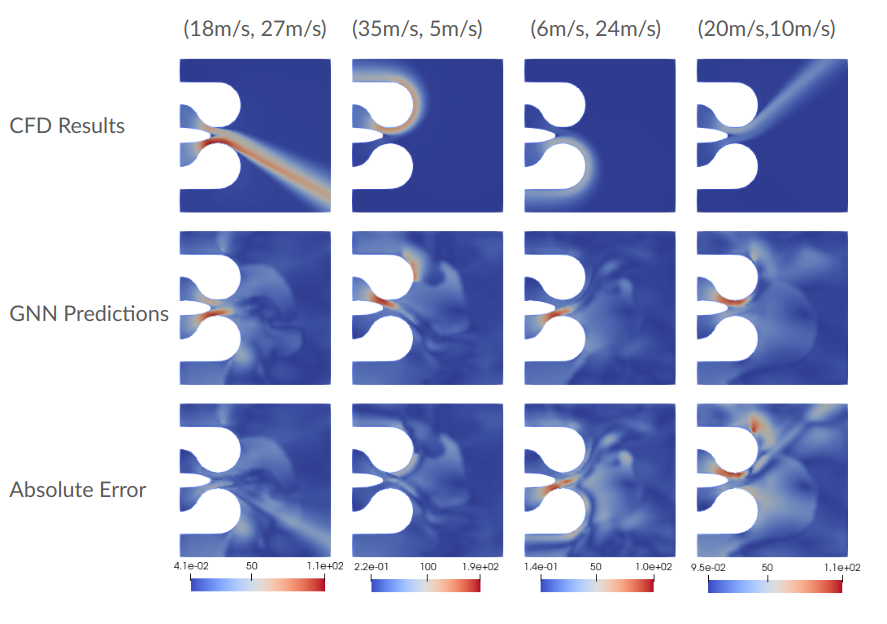
\includegraphics[width=14cm]{images/Methodology/Baselineprediction.png}
    \caption{Visualization of velocity fields for four cases from the baseline's prediction task, with inlet velocity values prescribed as (Inlet 1, Inlet 2) presented in four columns. Here, the first row represents results the target data, the second row corresponds to the GNN predictions for the velocity field, and the last row is the absolute difference between the target data and GNN predictions. The colours signify the magnitude of velocity, as mapped by the legend.} 
    \label{blpred}
\end{figure}
\begin{table}[ht]
    \centering
    \caption{Model evaluation metrics of the Baseline model for the reconstruction and prediction tasks. Here, "Abs. diff." refers to the absolute difference between the input and target data"} 
    \label{table:perform}
    \begin{tabular}{|l|l|l|l|l|}
    \hline
    \textbf{Model} & \textbf{Training Loss} & \textbf{Validation Loss} & \textbf{Test Loss} & \textbf{Abs. diff.} \\
    \hline
    Baseline - Reconstruction & 0.025627 & 0.028391 & 0.029312 & 0\\
    \hline
    Baseline - Prediction & 0.1459 & 0.1503 & 0.1635 & 0.2626\\
    \hline
    \end{tabular}
    \end{table}  
% As we can understand from the figure, the behavior of the outflow jet as well as its magnitude vary significantly from the expected target data. Thus, the baseline model is not feasible for the prediction task of nozzle flow dynamics.
Some important observations are: 
\begin{enumerate}
    \item  These loss values suggest that the model is generalizing reasonably well, although there's a slight increase in the test loss, indicating potential overfitting or high model variance when exposed to new data.
    \item For the different flow conditions presented, the model has successfully captured the essential flow patterns, as indicated by the similarity in the flow structures in CFD results and the predictions.
    \item The errors are localized to specific areas, particularly around the regions of flow separation and attachment.
    \item The smoother predictions in the GNN output compared to the sharper features in the CFD results could be indicative of numerical dissipation in the neural network’s processing.
\end{enumerate}
Thus, the model generally captures the flow patterns accurately across various conditions, as shown by the similarity in the large-scale flow features in the CFD and GNN results. Moreover, the errors are localized and do not dominate the entire flow field, indicating that the model's predictions are quantitatively close to the actual CFD results. The model has learned to approximate the fluid dynamics involved with a fairly good degree of accuracy given the proximity of the training, validation, and test losses. The slightly higher test loss points to the need for careful evaluation of the model's generalization capabilities. 
\subsection{Limitations}
Originally designed for small graphs with around 100 nodes, Graph U-Nets relies on dense matrix multiplications, which are memory-intensive and not scalable. This leads to memory constraints and slower training times, thus making it impractical for complex, large-scale graph data. GCNConv layers used in this architecture may have limited expressiveness in capturing higher-order graph structures and long-range dependencies in the graph. Its optimal depth is found to be 2 or 3 layers \cite{kipf}. Deeper models beyond 7 layers can encounter training difficulties due to the risk of overfitting. Apart from these issues, there is also a lack of a dedicated upsampling layer in the architecture, which leads to poor reconstruction of the latent space. Due to these disadvantages, Graph U-Net may exhibit poor performance in terms of both accuracy and efficiency, particularly for complex geometries or large datasets. Hence, there is a paramount necessity to rely on modified GNN architectures for our work.
\section{Proposed architecture}
\label{proparch}
In this section, we propose three GNN surrogate models and elucidate the architecture and improvements made to the original Graph U-Net framework. Then, we proceed to provide details on the hyperparameters and other implementation specifics of the proposed models. Finally, we demonstrate the training process and share the prediction results obtained for the CFD application. The models are developed on the Pytorch deep learning framework using the Pytorch Geometric (PyG) library. Training and testing are performed on a compute node of the \gls{HPC} cluster Loewenburg, using a single nVidia Tesla V100 GPU. \\
There are three different surrogate models proposed, and each of them tackles the unpooling limitation in Graph U-Net by using a \gls{k-NN} approach for upsampling used in PointNet++ \cite{pnpp}, with k set to 3. The downsampled features at different depths (levels of coarsening) are stored so that the upsampled node co-ordinates required for k-NN interpolation can be obtained from $[c_{x}, c_{y}]$ at the downsampled feature of the same depth. The architectures also include skip connections, although they do not perform the task of upsampling here. The three surrogate models differ in the convolutional operations used, as described below. 
\begin{enumerate}
    \item \textit{Graphknn} uses GCNConv layers as used in Graph U-Nets to perform convolutions and executes the upsampling operation with the help of k-NN interpolation. 
    \item The \textit{SAGEknn} surrogate model replaces the GCNConv layers of Graph U-Net with SAGEConv layers from GraphSAGE \cite{SAGE} and uses k-NN interpolation for unpooling. 
    \item In \textit{MoNetknn}, we carry out convolutions using the GMMConv layers from the MoNet \cite{MoNet} architecture, along with k-NN interpolation for upsampling. 

    % \item \textit{BL + crsn + knn:} In this surrogate, we first obtain the set of coarsened meshes through incremental decimation of the CFD mesh by running a Python script on Paraview. With the mesh indices and co-ordinates of the low-resolution mesh nodes, we compute the downsampled features for the graph using the sampling operator described in the subsection \ref{SO}. Thus, we implement the pooling operation with the help of sampling operator and perform unpooling operation using k-NN interpolation. 
    % \item \textit{BL + SAGE + crsn + knn:} Similar to the previous model in every detail, the only difference in this model is that it uses GraphSAGE layers instead of the GCNConv layers as convolutions.
    % \item \textit{BL + MoNet + sampl. + knn:} This model is also similar to \textit{BL + crsn + knn}, but it applies MoNet blocks for up convolutions and down convolutions. 
\end{enumerate}
We perform hyperparameter tuning for each of the architectures to arrive at the ideal choice of design parameters. All the models showcase their best performance for the same hyperparameter configuration - 48 channels, 3 hidden layers each with a pooling ratio of 0.5, ReLU activations and weights initialized by the Kaiming method. We use a batch size of 4 and set up the initial learning rate as 0.0005, to be used along with a Step LR scheduler similar to the baseline surrogates. We use the Adam optimizer and train on the RMSE loss. 
% The salient features of the three architectures along with their hyperparameters are tabulated in Table \ref{prophp}. 
% % \subsection{Multi-Resolution Graph Net Architecture}
% % \section{Model hyperparameters and training parameters}
% \begin{table}[ht]
%     \centering
%     \caption{Features and hyperparameters comparison of 1. \textit{Graphknn}, 2. \textit{SAGEknn}, and 3. \textit{MoNetknn} architectures.}
%     \label{prophp}
%     \begin{tabular}{|l|l|l|l|}
%     \hline
%     \textbf{Feature/Hyperparameter}    & \textit{Graphknn} & \textit{SAGEknn}   & \textit{MoNetknn} \\
%     \hline
%     Channels    & 48 & 48 & 48                           \\
%     \hline
%     Hidden layers    & 3 & 3 & 3                          \\
%     \hline
%     Convolution layer             &     GCNConv & SAGEConv & GMMConv                   \\
%     \hline
%     Pooling operation             &    Top-k &  Top-k &  Top-k                     \\
%     \hline
%     Unpooling operation         &   k-NN&   k-NN &   k-NN               \\
%     \hline
%     Batch size                 & 4 & 4& 4                         \\
%     \hline
%     Activation function        & ReLU  & ReLU  & ReLU                       \\
%     \hline
%     Weight initialization    &  Kaiming &  Kaiming &  Kaiming                        \\
%     \hline
%     Initial learning rate       & 0.0005 & 0.0005 & 0.001                        \\
%     \hline
%     \end{tabular}
%     \end{table}
\section{Results and discussion}
We perform a 9-fold cross-validation on the training and validation datasets. Figures \ref{2vel1} and \ref{2vel2} depict the predicted velocity fields and the associated absolute errors obtained from the three surrogates for four different flow conditions. Figure \ref{aloop} provides an overview of the predicted pressure and velocity fields for all the surrogate models discussed here for a case showing Coanda adhesion. \\
\begin{figure}[ht]
    \centering
    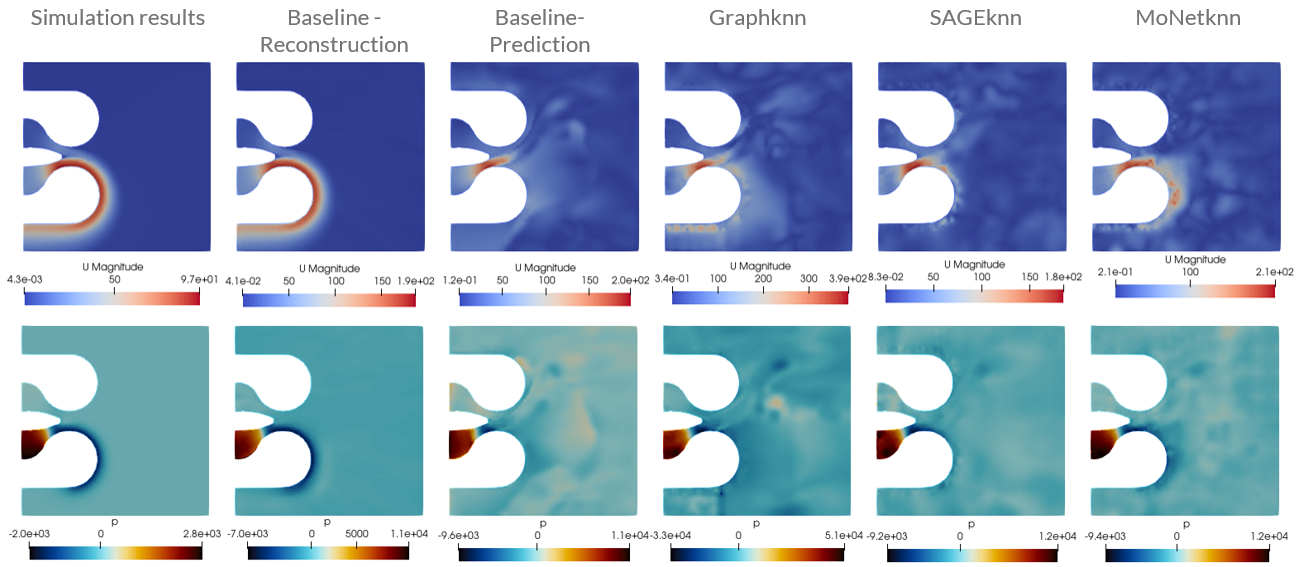
\includegraphics[width=15cm]{images/Methodology/presvelcomp.png}
    \caption{Predicted velocity and pressure fields for the case with (Inlet 1, Inlet 2) = (35 m/s, 5 m/s). The leftmost column represents simulation results, whereas the subsequent columns correspond to the predictions of the respective architectures.} 
    \label{aloop}
\end{figure}
\begin{figure}[ht]
    \centering
    \begin{subfigure}[b]{14cm}
        \centering
        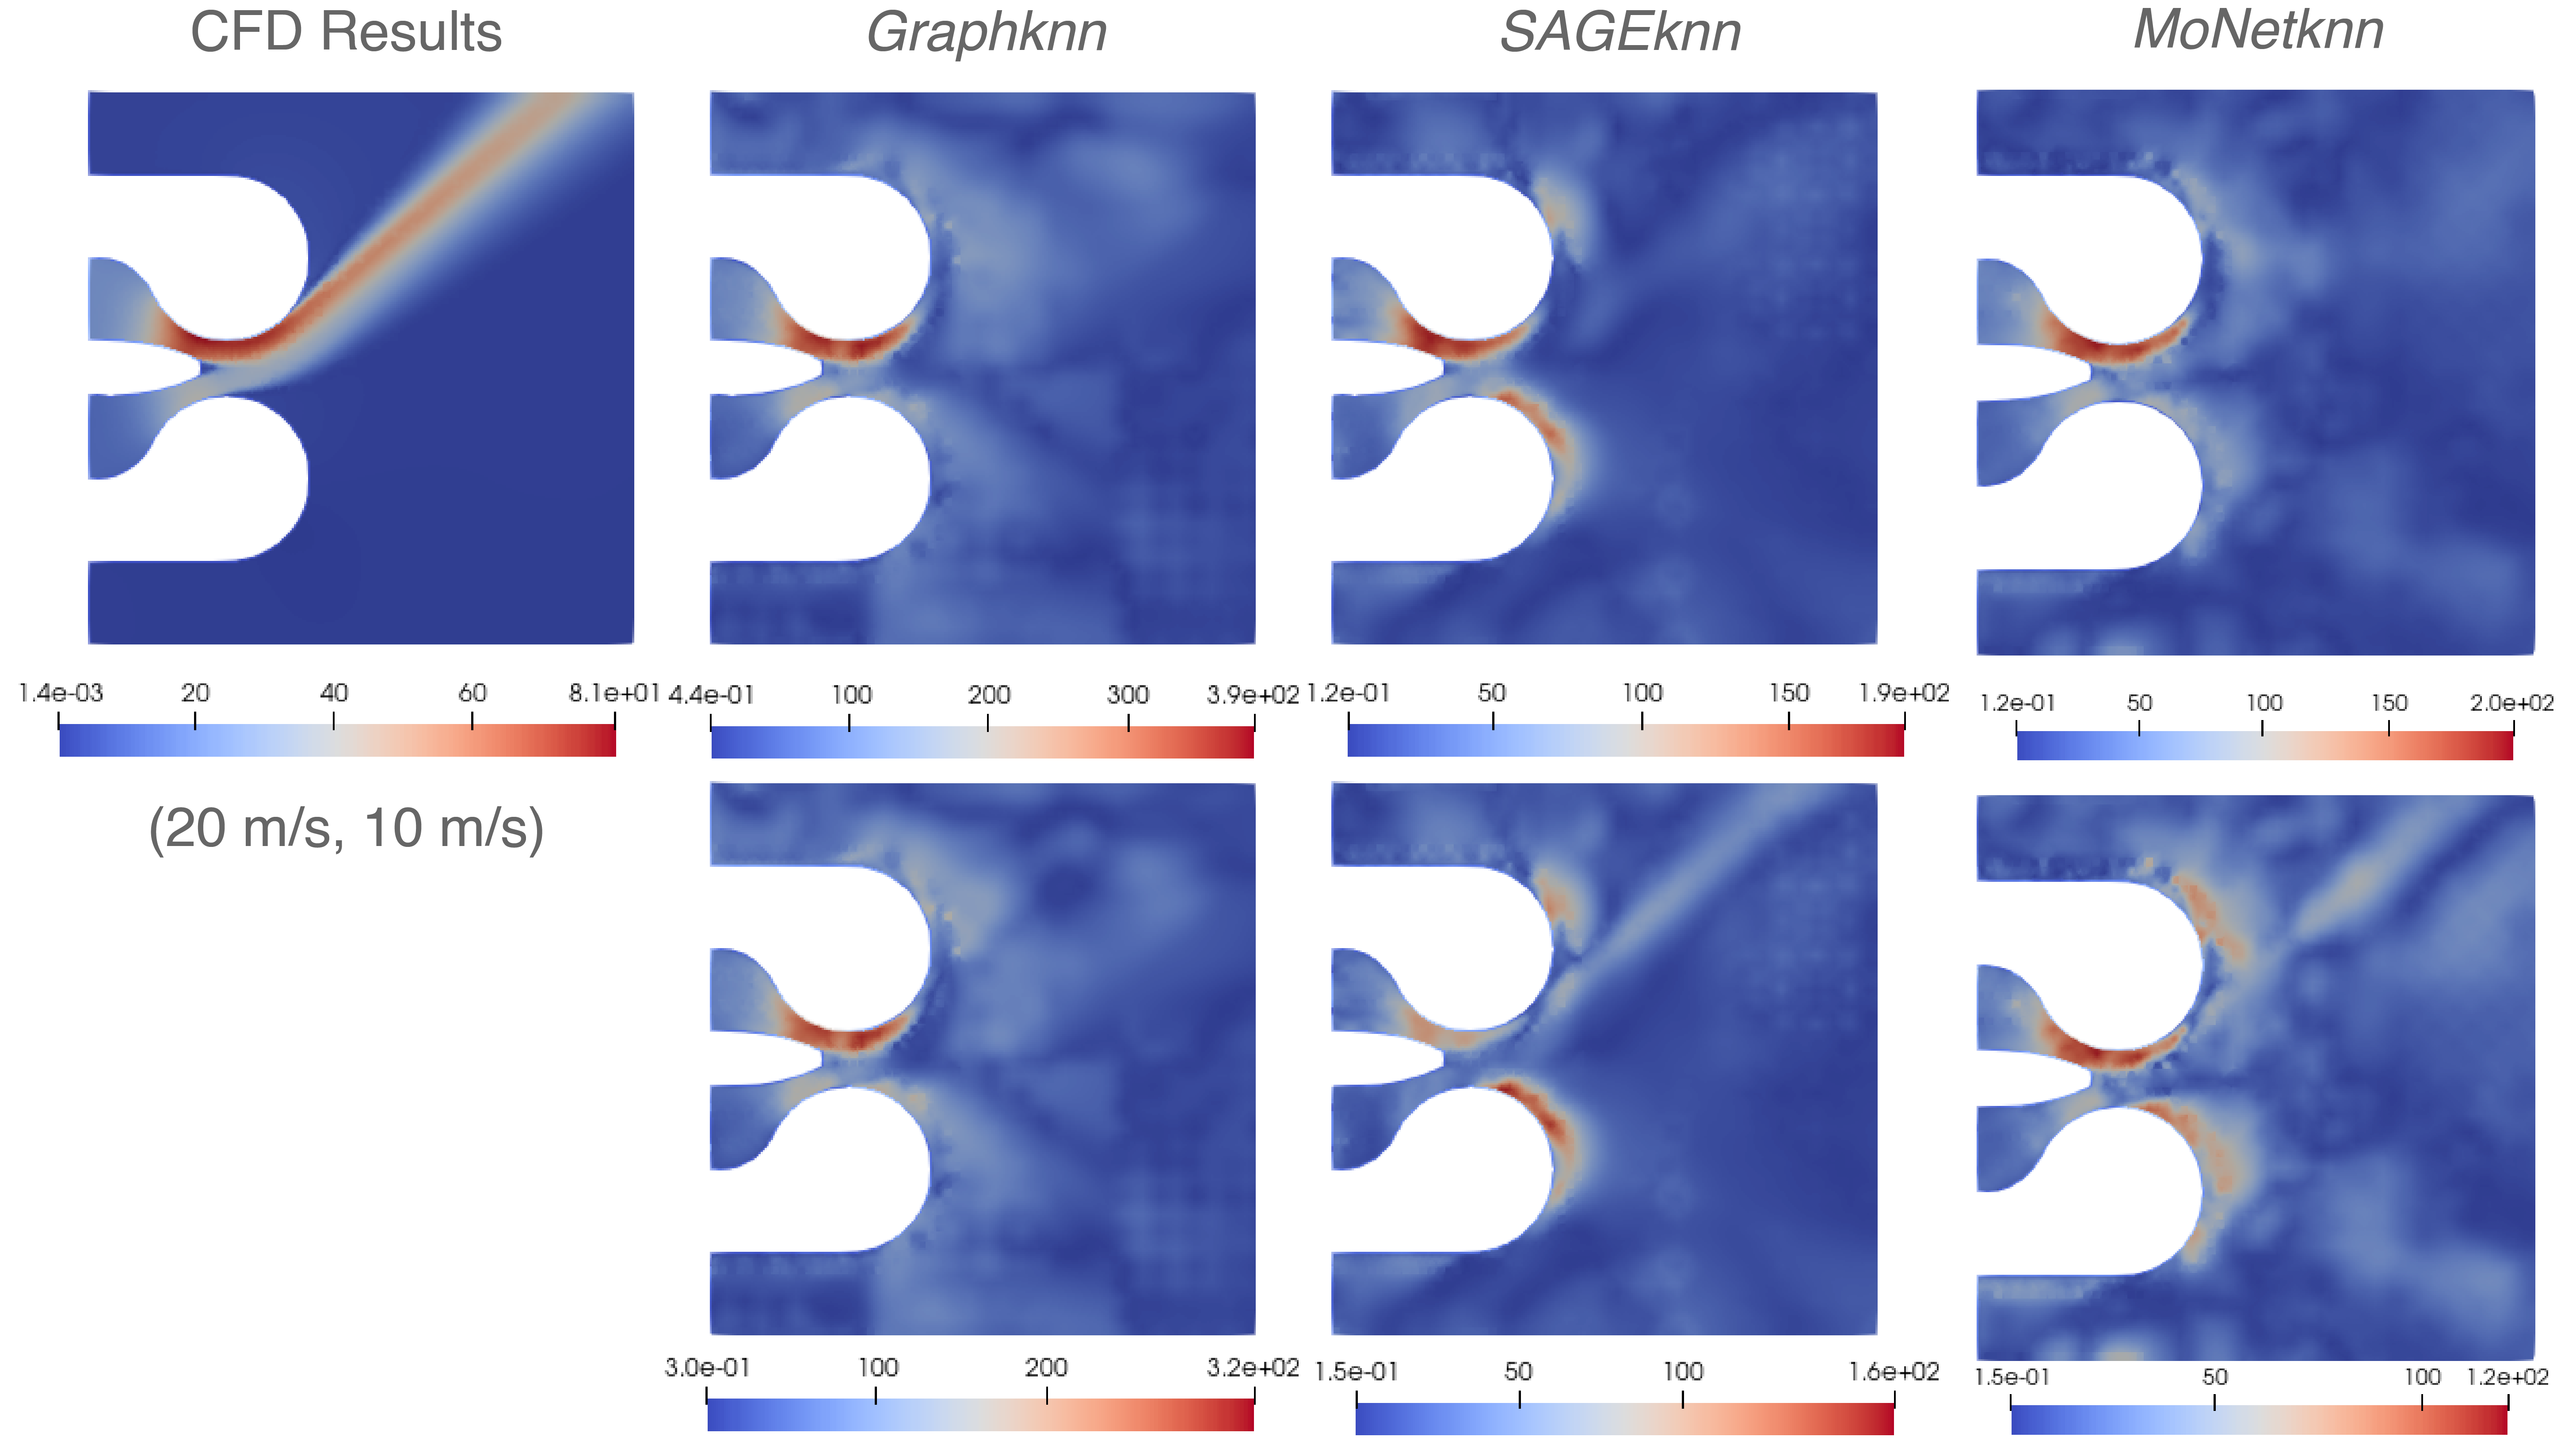
\includegraphics[width=\textwidth]{images/Methodology/Asset 18.png}
        \caption{Case (20 m/s, 10 m/s) showing jet deflection to the top Coanda surface.}
        \label{fig:allvel1}
    \end{subfigure}
    % \vspace{2.5cm} % Adds some vertical space between the subfigures
    \begin{subfigure}[b]{14cm}
        \centering
        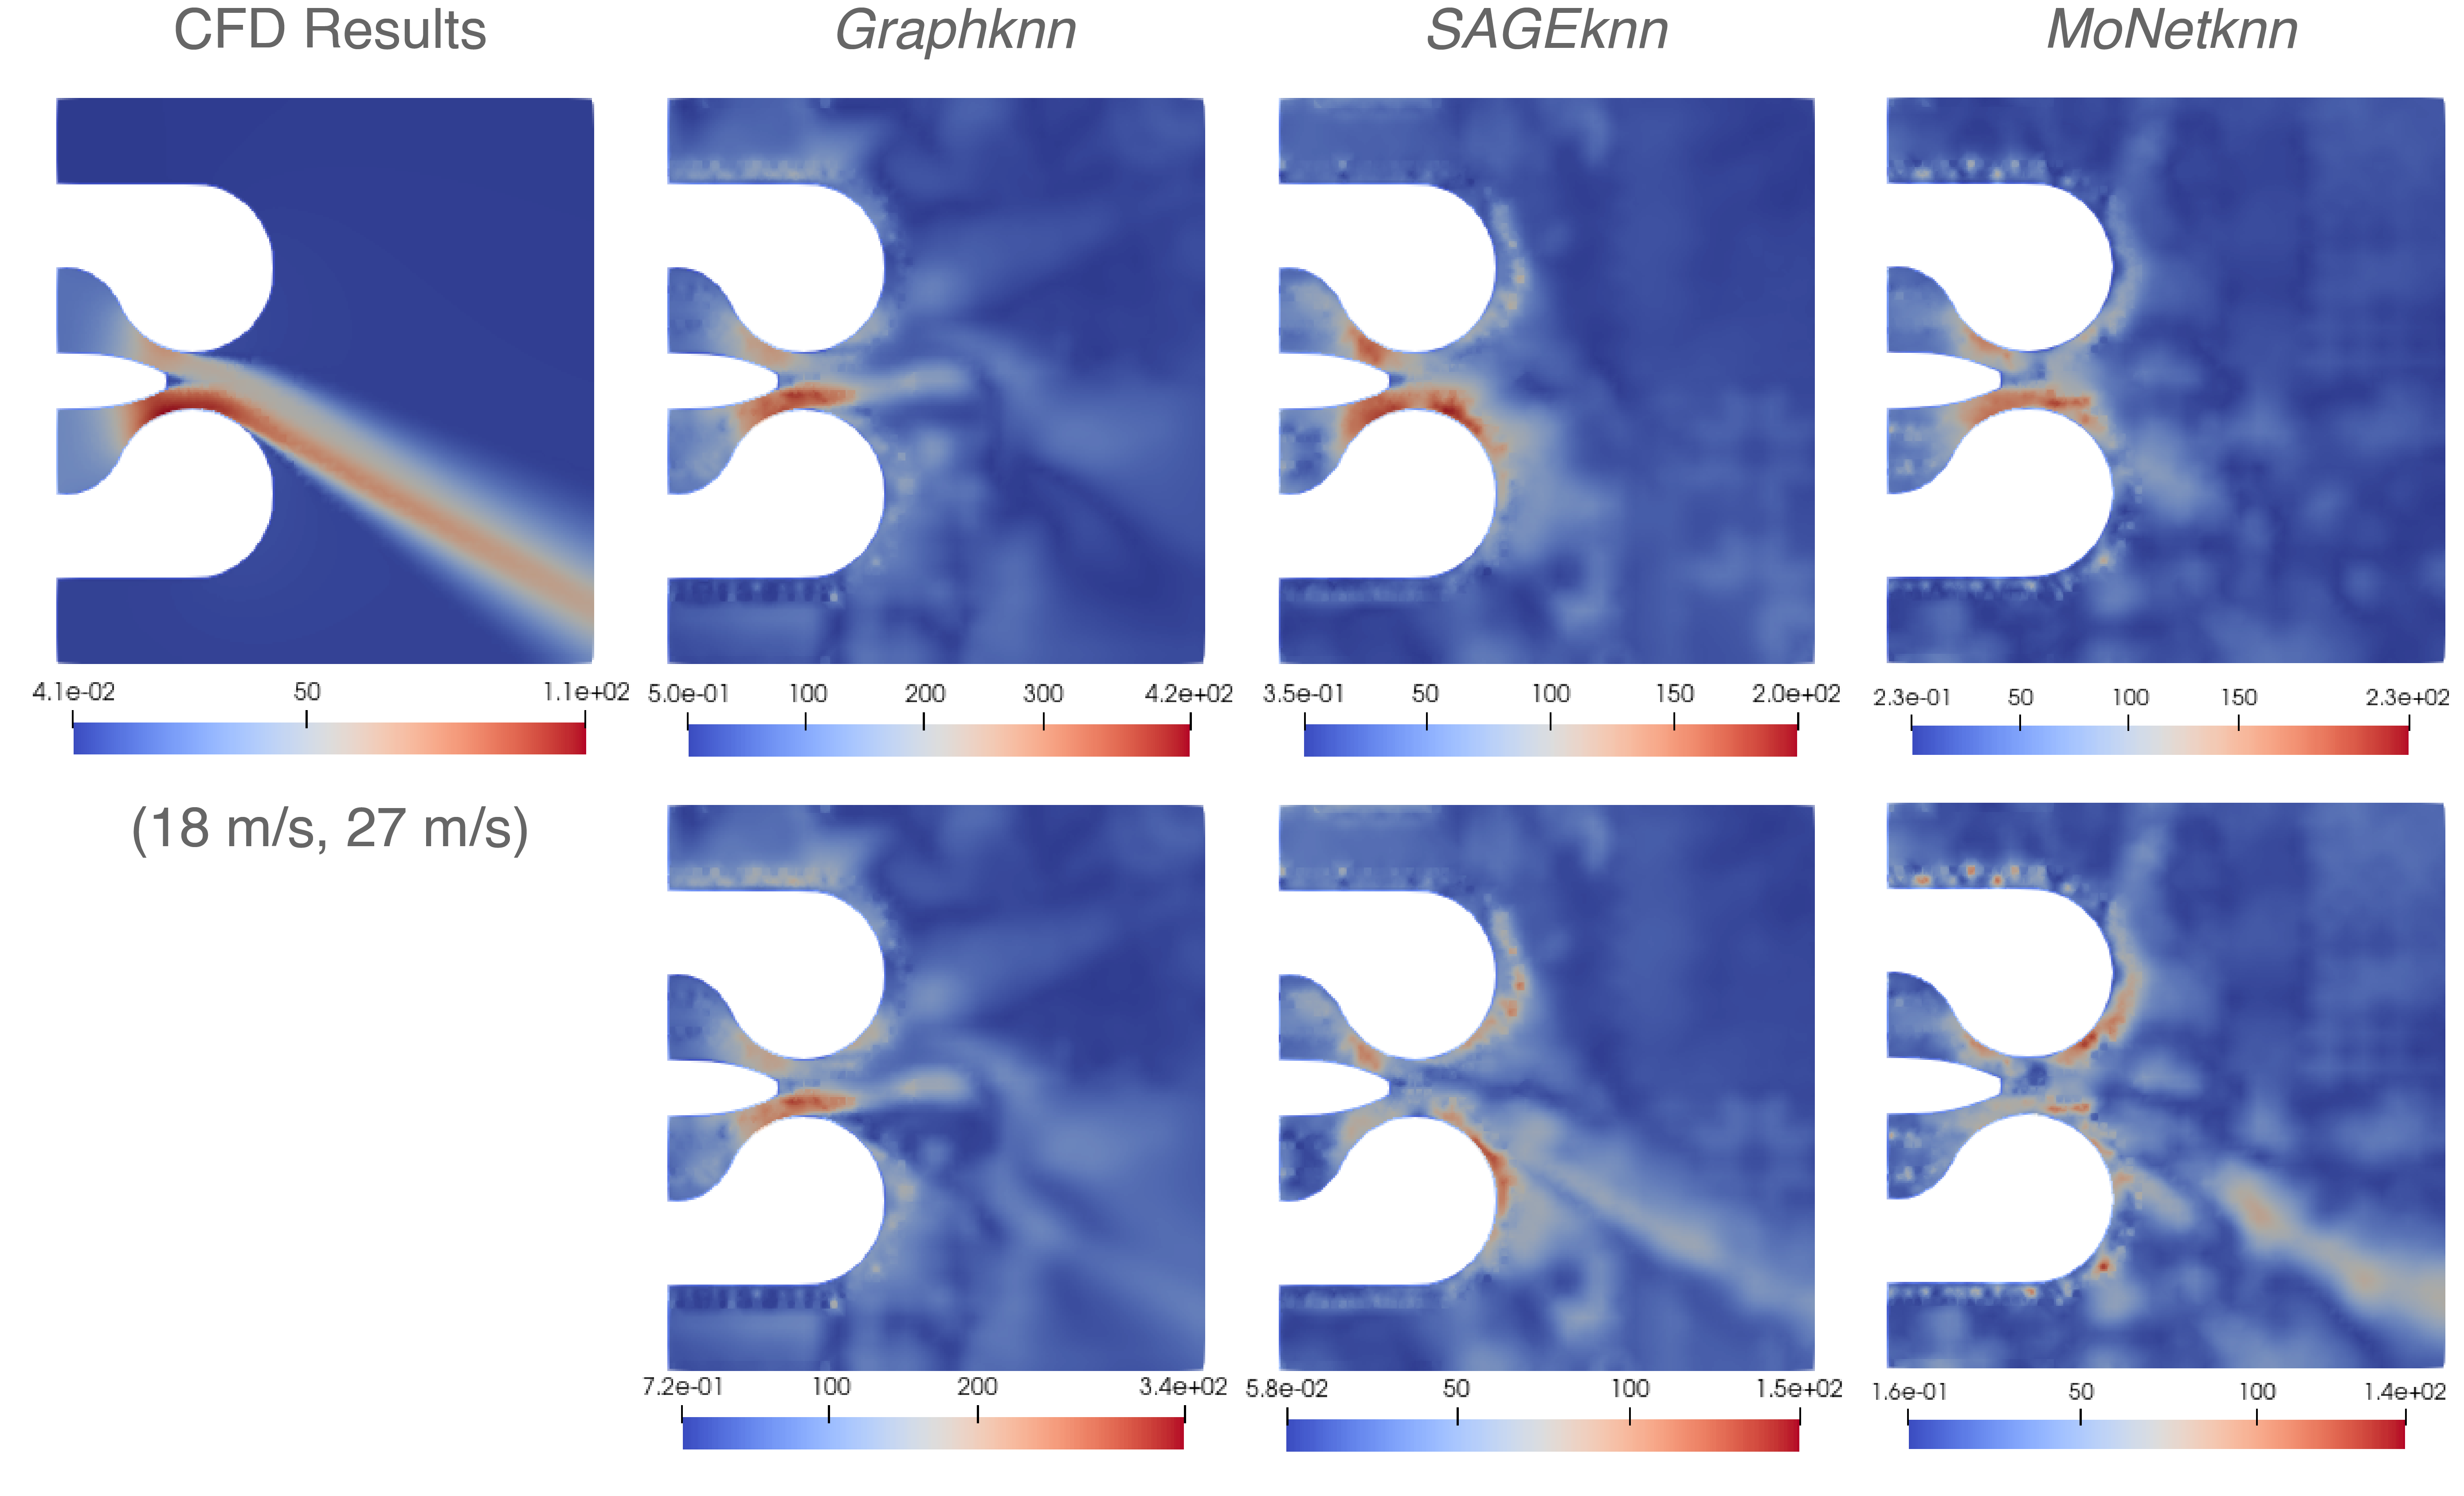
\includegraphics[width=\textwidth]{images/Methodology/Asset 17.png}
        \caption{Case (18 m/s, 27 m/s) showing jet deflection to the bottom Coanda surface.}
        \label{fig:allvel2}
    \end{subfigure}
    % \vspace{-10mm} % Adds some vertical space between the subfigures
    \caption{Visualization of velocity fields for two cases with inlet velocities (Inlet 1, Inlet 2): the first row depicts the predictions, and the second row shows the absolute difference between the target and predictions. The top left corner presents the simulation results.}
    \label{2vel1}
\end{figure}
\begin{figure}[ht]
    \centering
    \begin{subfigure}[b]{14cm}
        \centering
        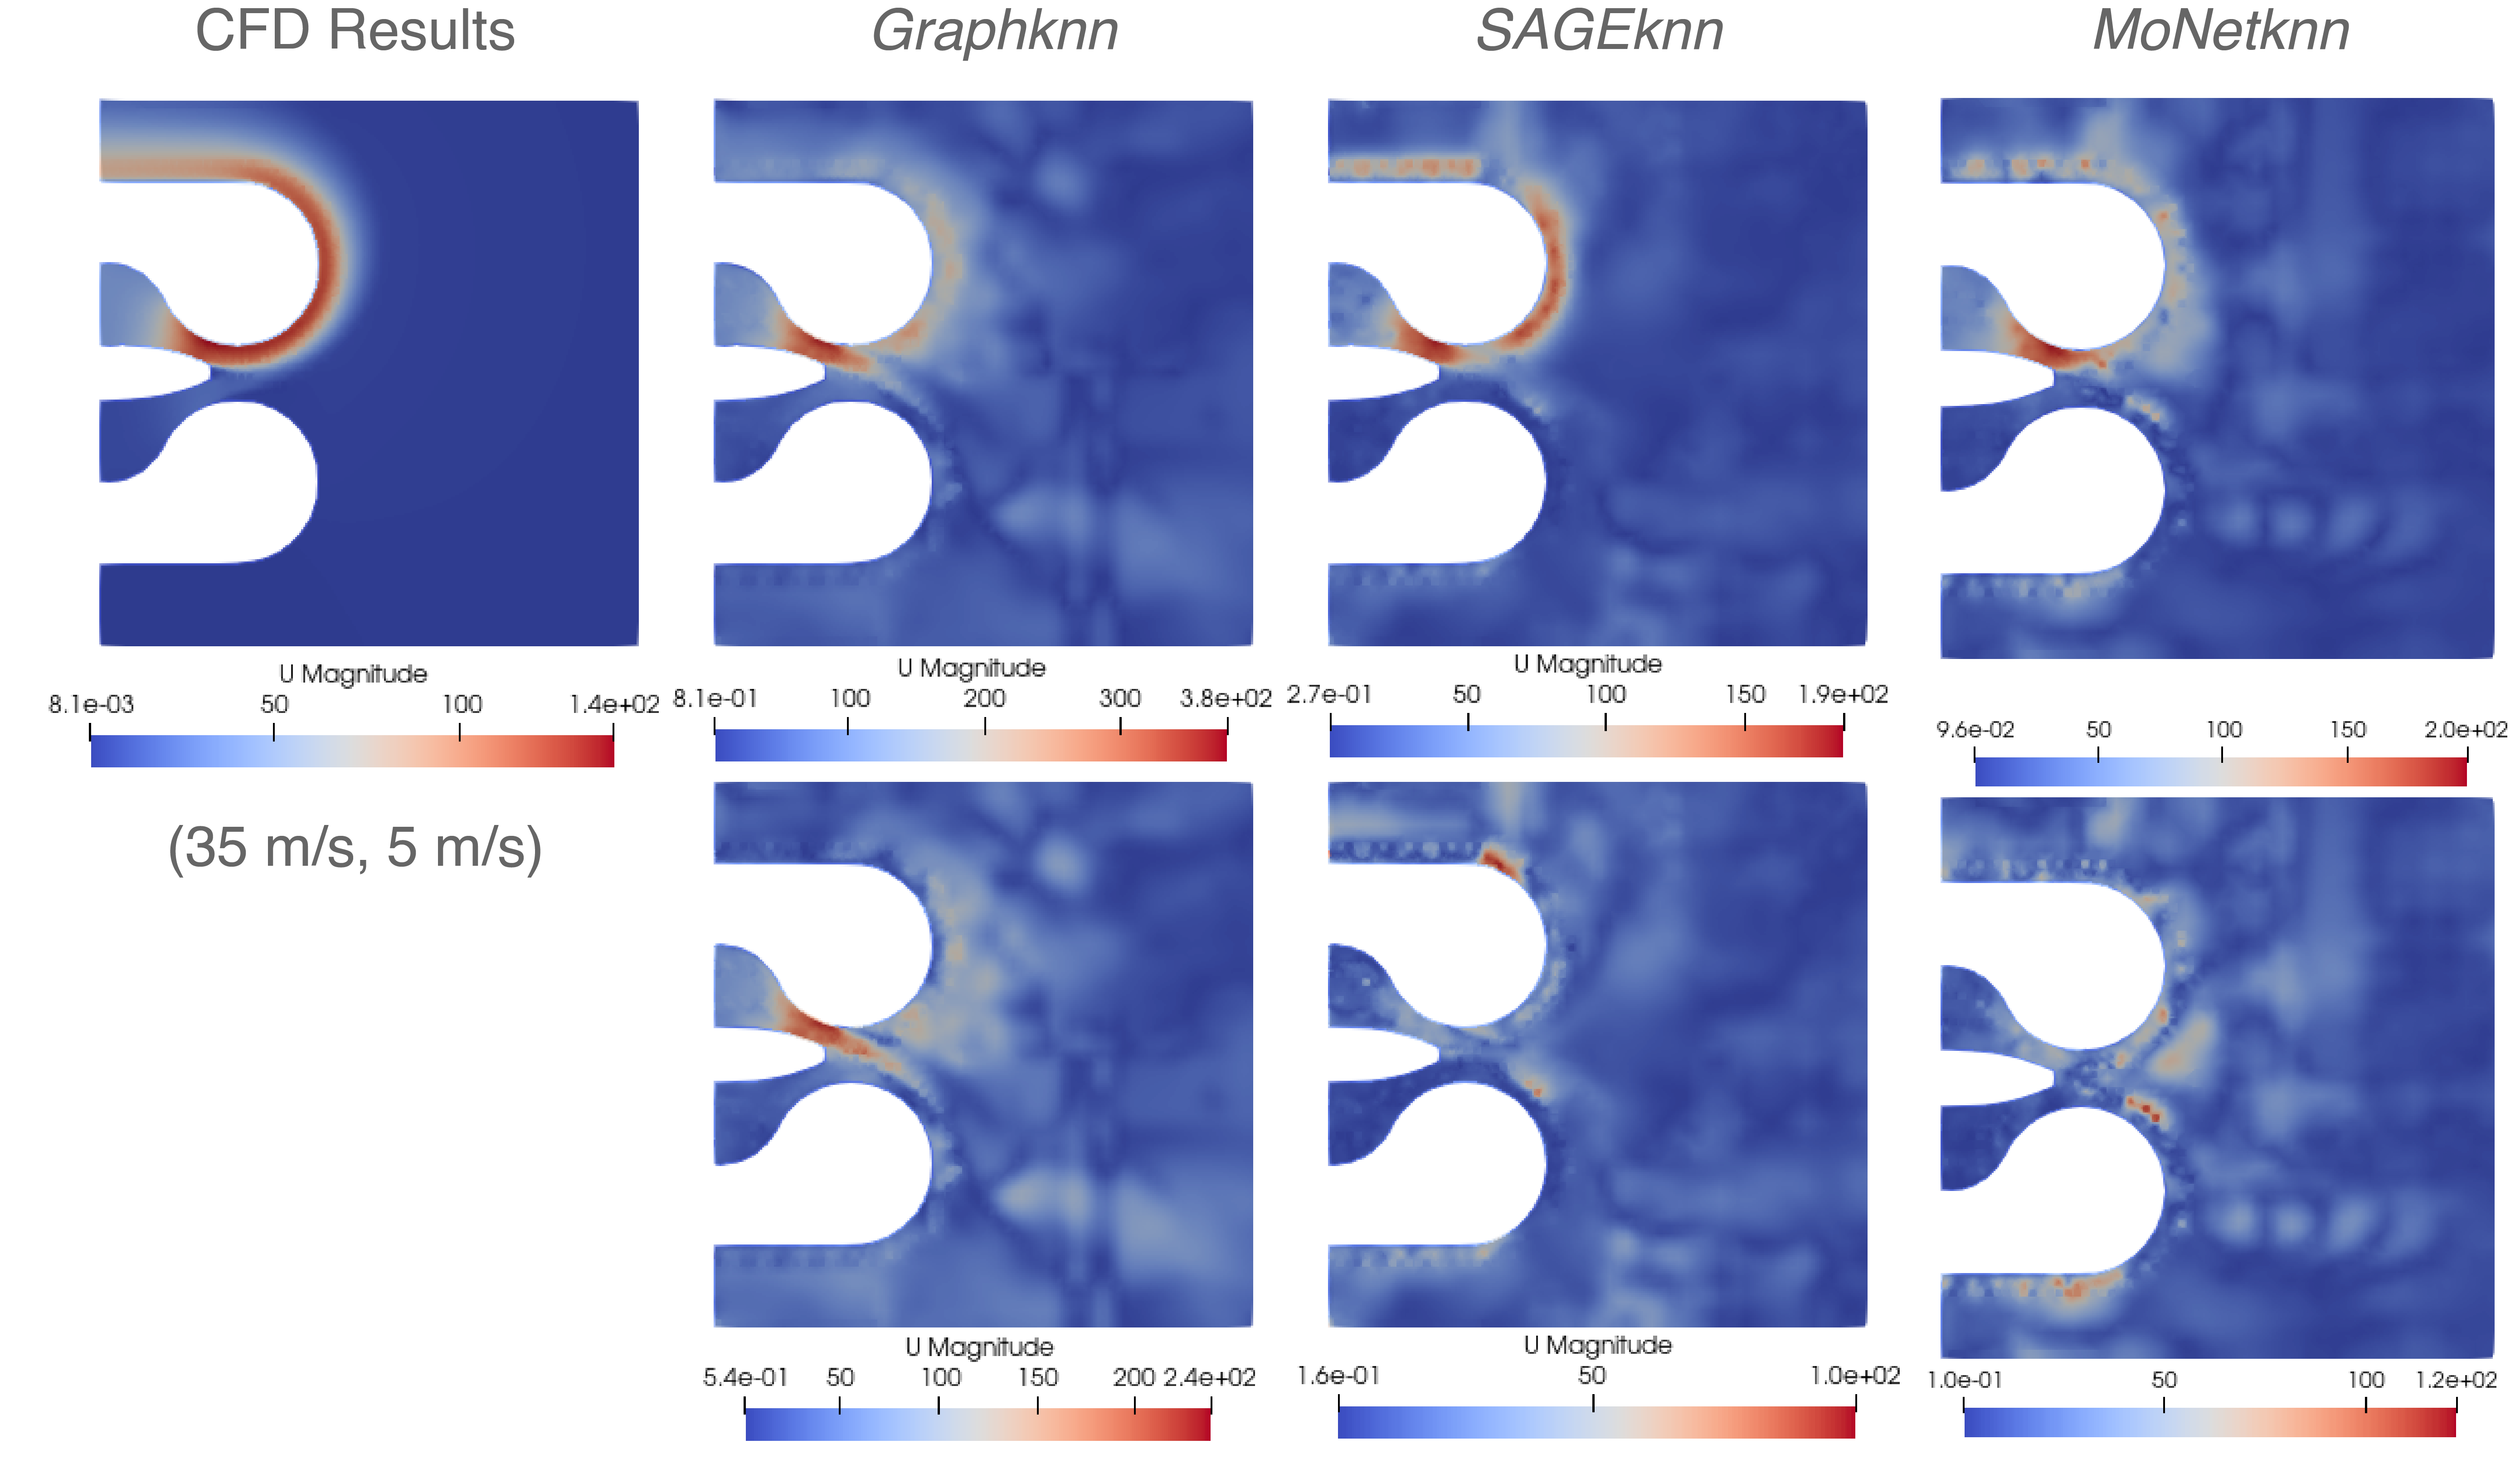
\includegraphics[width=\textwidth]{images/Methodology/Asset 15.png}
        \caption{Case (35 m/s, 5 m/s) showing complete adhesion to the top Coanda surface.}
        \label{fig:allvel3}
    \end{subfigure}
    % \vspace{2.5cm} % Adds some vertical space between the subfigures
    \begin{subfigure}[b]{14cm}
        \centering
        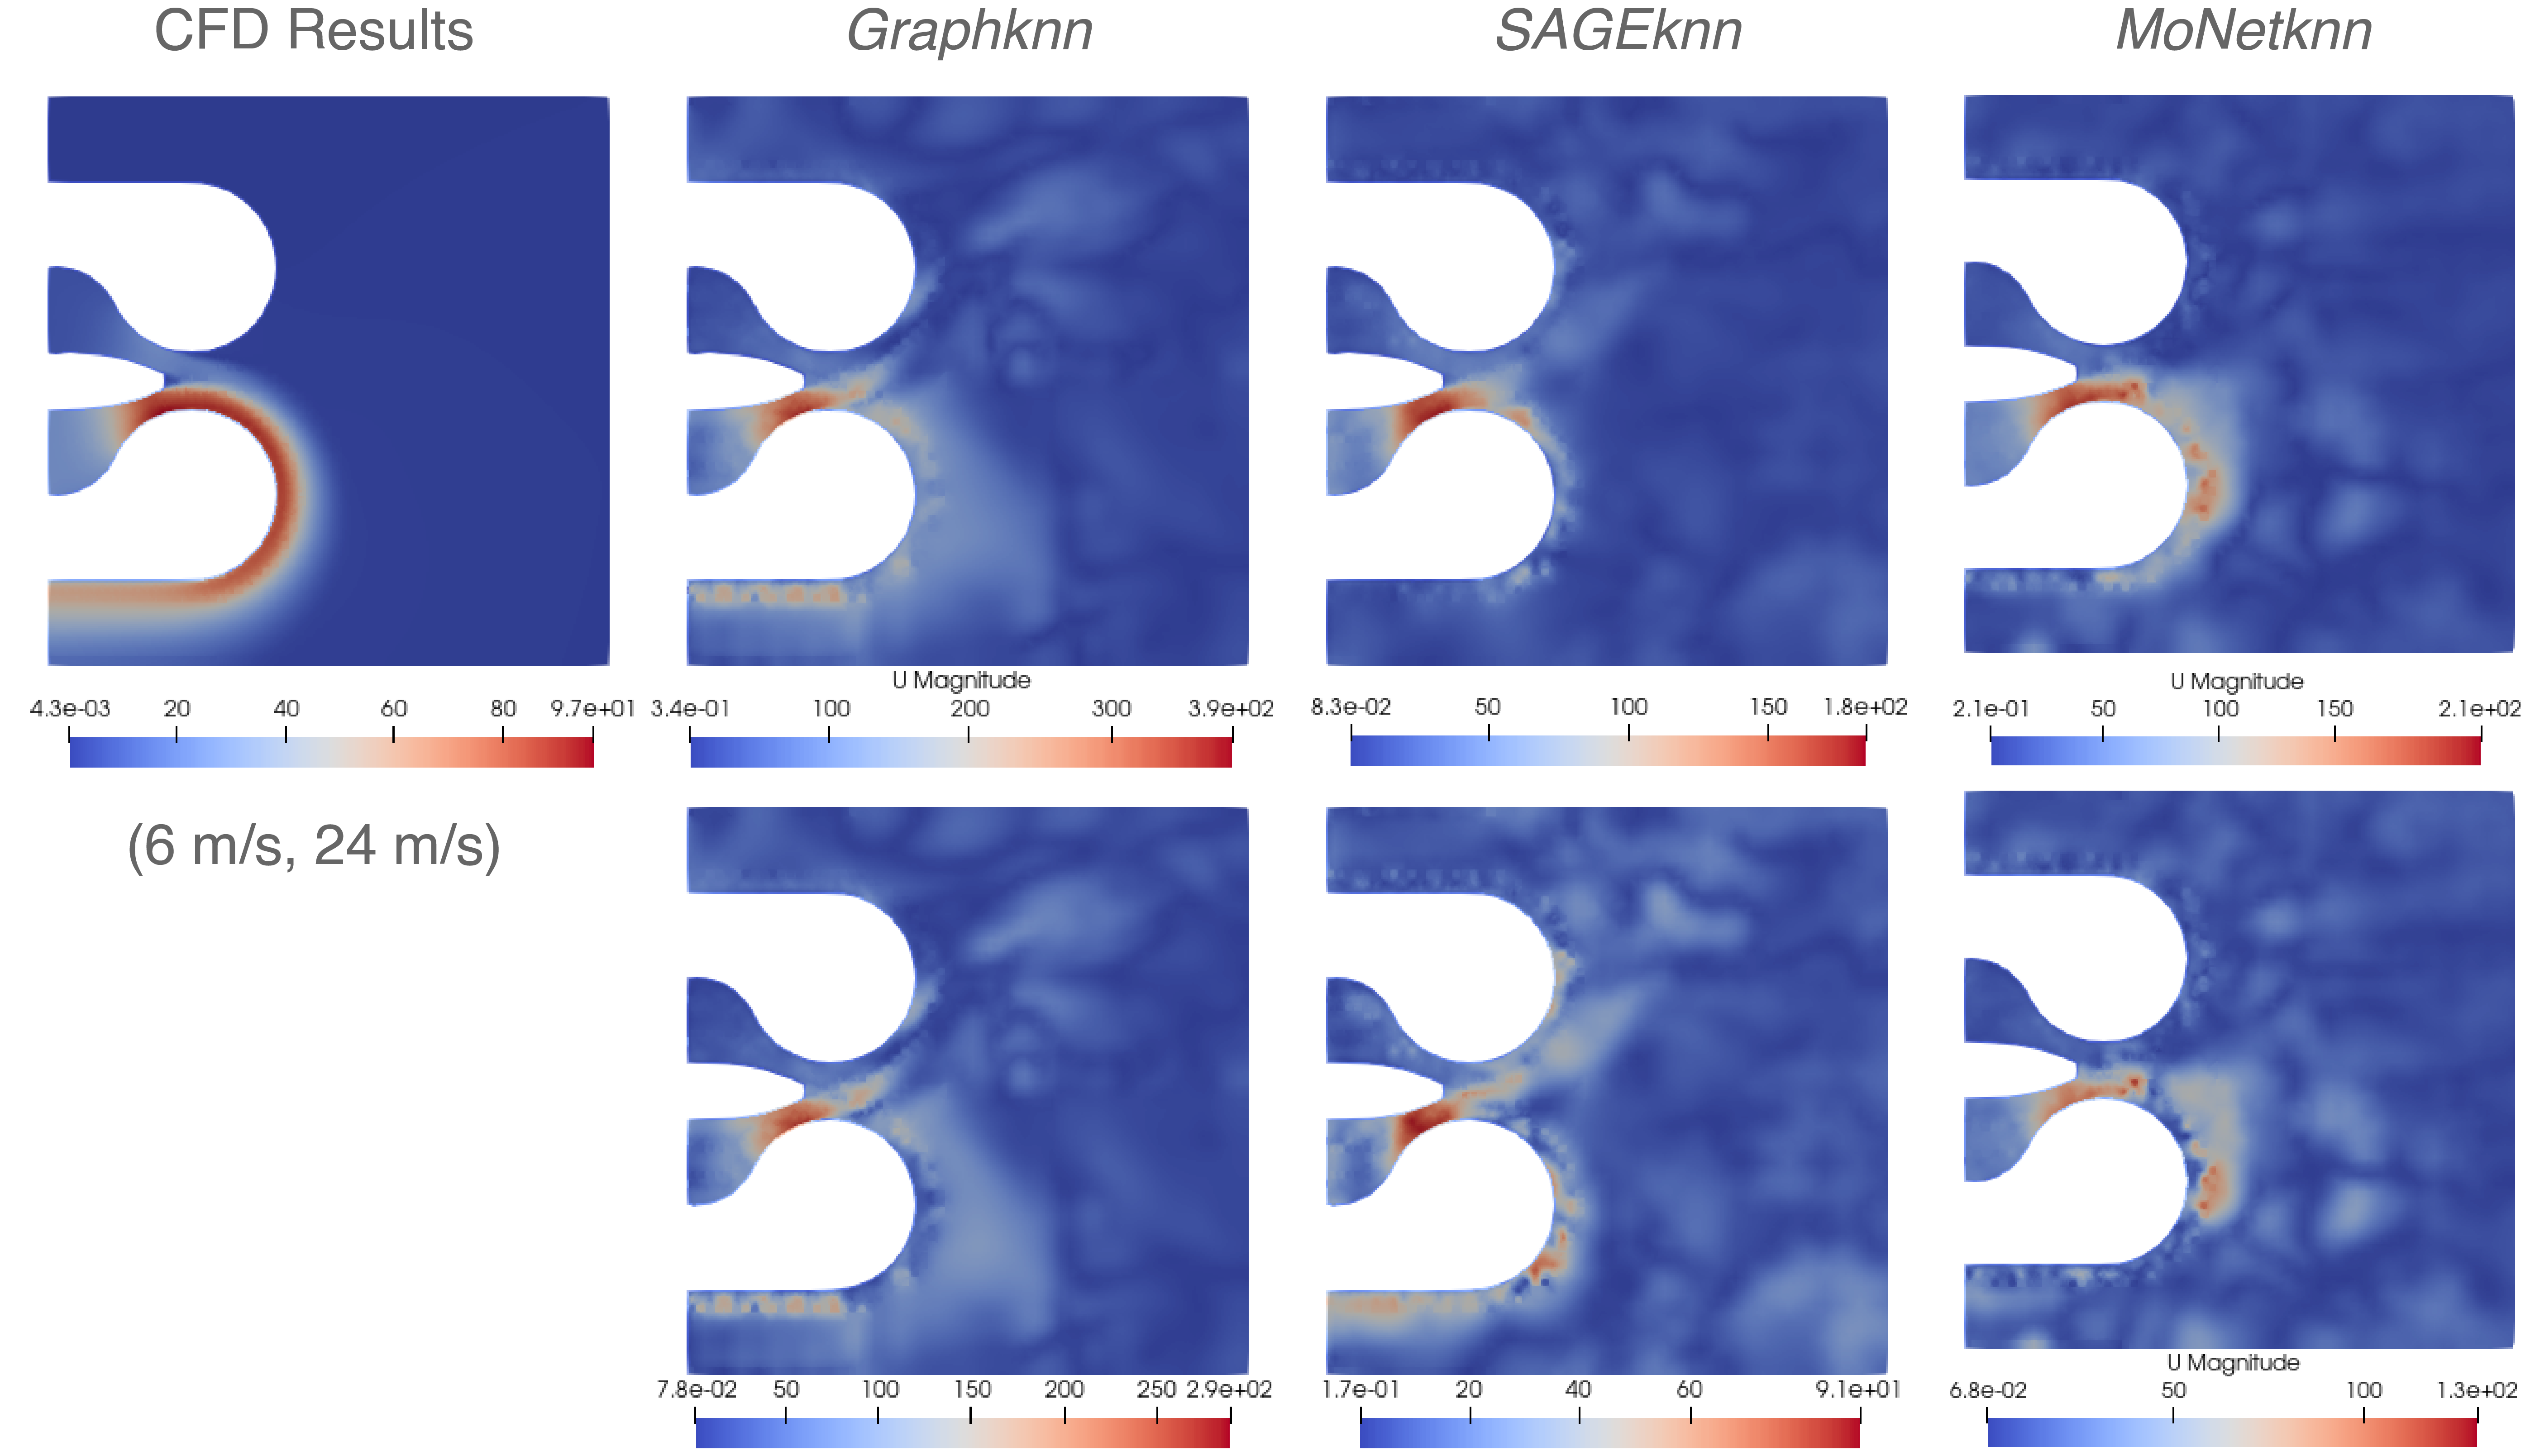
\includegraphics[width=\textwidth]{images/Methodology/Asset 14.png}
        \caption{Case (6 m/s, 24 m/s) showing complete adhesion to the bottom Coanda surface.}
        \label{fig:allvel4}
    \end{subfigure}
    % \vspace{-10mm} % Adds some vertical space between the subfigures
    \caption{Visualization of velocity fields for two cases with inlet velocities (Inlet 1, Inlet 2): the first row depicts the predictions, and the second row shows the absolute difference between the target and predictions. The top left corner presents the simulation results.}
    \label{2vel2}
\end{figure}
We note that the duration of steady-state simulations is extremely long, about 8.5 hours. Note that roughly eight cases are concurrently processed on the Loewenburg HPC cluster with an Intel Xeon Gold 6130F \gls{CPU}, running at a base frequency of 2.10 GHz. Subsequent simulation cases queued and initiated as prior ones conclude using the \gls{SLURM} scheduler. A simulation takes around 32 minutes on average in the parallel configuration of \verb |OpenFOAM|, amounting to around 8.5 hours for the cumulative simulations of 120 cases. \\
Investigating further into the test cases, we compute the test loss of each sample in the test dataset and tabulate them in Table \ref{t:}.
% To discern the performance of these models, we compute the RMSE loss over the training, validation and test datasets, observed in Table \ref{t:predloss}. We observe that the \textit{MoNetknn} architecture performs slightly better than \textit{SAGEknn} which is marginally superior to \textit{Graphknn} in terms of training loss. While \textit{Graphknn} surpasses the other two models in terms of test loss, \textit{SAGEknn} proves to be the relatively better model to \textit{MoNetknn} on the test dataset. Furthermore, we also monitor the training and test times of the three models along with the time taken to batch execute the CFD simulations, presented in Table \ref{t:times}. 
\begin{table}[ht]
    \centering
    \caption{Evaluation metrics of  1. \textit{Graphknn}, 2. \textit{SAGEknn}, and 3. \textit{MoNetknn} architectures. } 
    \label{t:predloss}
    \begin{tabular}{|l|l|l|l|}
    \hline
    \textbf{Model} & \textbf{Training Loss} & \textbf{Validation Loss} & \textbf{Test Loss}\\
    \hline
     \textit{Graphknn} & 0.134412& 0.143149 & 0.136981   \\
    \hline
    \textit{SAGEknn}& 0.123704 & 0.138665 & 0.133959 \\
    \hline
    \textit{MoNetknn} & 0.129066  & 0.138896 & 0.146817  \\
    \hline
    \end{tabular}
\end{table}
% \begin{table}[ht]
%     \centering
%     \caption{Time taken for training and testing of  1. \textit{Graphknn}, 2. \textit{SAGEknn}, 3. \textit{MoNetknn} models, 4. Transition, and 5. Steady-state simulations.} 
%     \label{t:times}
%     \begin{tabular}{|l|l|l|l|l|l|}
%     \hline
%     \textbf{Model} & \textit{Graphknn} & \textit{SAGEknn} & \textit{MoNetknn} & Transition & Steady-state \\
%     \hline
%     Training time (hours) & 3.88 & 3.2& 4.15  & 8.5 & 0.3 \\
%     \hline
%     Test time (seconds) & 0.09157  & 0.09382 & 0.09413 & -& - \\
%     \hline
%     \end{tabular}
% \end{table}
\begin{table}[ht]
    \centering
    \caption{Time taken for training and testing of  (1) \textit{Graphknn}, (2) \textit{SAGEknn}, (3) \textit{MoNetknn} models, (4) Transition, and (5) Steady-state simulations. Note that the training time for (4) and (5) refers to simulation times.} 
    \label{t:times}
    \begin{tabular}{|l|l|l|}
    \hline
    \textbf{Setup}& \textbf{Training time (hours)} & \textbf{Test time (seconds)} \\
    \hline
    \textit{Graphknn} & 3.88 & 0.09157 \\
    \hline
    \textit{SAGEknn} & 3.2 & 0.09382 \\
    \hline
    \textit{MoNetknn} & 4.15 & 0.09413 \\
    \hline
    Steady-state& 8.5 & - \\
    \hline
    Transition & 0.3 & - \\
    \hline
    \end{tabular}
\end{table}
% From the visual inspection of each of the s
\begin{table}[ht]
    \centering
    \caption{Individual loss estimation of test samples in 1. \textit{Graphknn}, 2. \textit{SAGEknn}, 3. \textit{MoNetknn} models and identification of noisy data (highlighted in red). For each test case, the value in bold corresponds to the best test loss achieved out of the three models. The average test loss, excluding noise data, is also computed and the best prediction case for each model are stated.}
    \label{t:}
    \begin{tabular}{|l|l|l|l|}
        \hline
        \textbf{Case No. (Inlet 1, Inlet 2)} & \textit{Graphknn} & \textit{SAGEknn} & \textit{MoNetknn} \\
        \hline
        10 (18 m/s, 27 m/s)& 0.1627682& \textbf{0.141760} & 0.161019\\
        \hline
        \rowcolor{red!30}\textbf{85 (45 m/s, 20 m/s)} & 0.227854 & \textbf{0.294137} & 0.256933\\
        \hline
        96 (45 m/s, 10 m/s)& 0.146616 & 0.153643 & 0.158489 \\
        \hline
        115 (27 m/s, 3 m/s)& 0.111698& \textbf{0.100347} & 0.116409 \\
        \hline
        93 (32 m/s, 8 m/s)& 0.1099330 & \textbf{0.095786} & 0.125213 \\
        \hline
        31 (6 m/s, 24 m/s) & 0.115487& \textbf{0.073103} & 0.108589 \\
        \hline
        94 (36 m/s, 9 m/s)& 0.130061 & \textbf{0.120798} & 0.152372 \\
        \hline
        88 (15 m/s, 5 m/s)& \textbf{0.123582} & 0.133565 & 0.128406 \\
        \hline
        97 (15 m/s, 3 m/s)& 0.134011 & \textbf{0.122433} & 0.144798 \\
        \hline
        110 (35 m/s, 5 m/s)& 0.111097 & \textbf{0.0962448} & 0.122681 \\
        \hline
        48 (3 m/s, 21 m/s)& \textbf{0.124982}& 0.135190 & 0.140194 \\
        \hline
        80 (20 m/s, 10 m/s)& 0.145688 & \textbf{0.140505} & 0.146698 \\
        \hline
        \textbf{Test Loss} & 0.136981 & \textbf{0.133959}& 0.146817\\
        \hline
        \textbf{Test Loss (w/o noise)} & 0.128720 & \textbf{0.119398} & 0.136806\\
        \hline
        \textbf{Best Case} & Case 93 & Case 31& Case 31\\
        \hline
    \end{tabular}
\end{table}
% This insight paves the way for targeted advancements in the \textit{SAGEknn} architecture, bolstering its potential to become a more precise tool for modeling nozzle flow dynamics. \\




% While steady-state simulations require extensive computational time, the synergy between GNN models and transitional simulations can effectively streamline the process. 
% Given the extremely long durations of steady-state simulations, performing the GNN training following the transitional simulations could significantly reduce the total simulation
% Thus, steady-state simulations  \\
% All three surrogates perform better than the baseline model in predicting the steady state solutions. From the comparative analysis of these metrics, we can conclude overall that \textit{SAGEknn} is the most efficient and accurate among the three surrogate models. Although all the surrogate models fail to capture the physics behind the turbulent steady-state solutions, this study has shown the most promising alternative for Graph U-Net in this context, which is \textit{SAGEknn}. Thus, further investigation and improvement can be done on the \textit{SAGEknn} architecture to enhance the predictive accuracy of the model for nozzle flow dynamics. 

% Continued refinement and development of \textit{SAGEknn} promise to yield further improvements in the fidelity of CFD simulations. Integration of physics-informed layers are anticipated to significantly augment the model's accuracy in capturing the complex phenomena of nozzle flow dynamics. \\
% The empirical results from the surrogate models demonstrate an enhanced predictive capability for steady-state solutions compared to the baseline model. Notably, the SAGEknn model distinguishes itself through its superior performance metrics, emerging as the most effective and precise in our comparative analysis. While all surrogate models exhibit limitations in fully encapsulating the turbulent physics characteristic of steady-state nozzle flows, SAGEknn offers the most promising framework for refinement.
% It is evident that the SAGEknn architecture, with its advanced graph convolution techniques, provides a strong foundation for further research. Future work will involve a deeper dive into the SAGEknn model's architecture to fine-tune and enhance its capacity to model the intricacies of turbulence. 
% Optimizations in areas such as convolutional layer design, activation functions,
\section{Key observations and inference}
We make the following key observations in regard to the evaluation metrics obtained: 
\begin{enumerate}
    \item  The comparative analysis reveals a positive trend: all three surrogate models exhibit superior performance over the baseline model in predicting steady-state solutions.
    \item \textit{SAGEknn} stands out as the most balanced model, offering both the best generalization performance (as indicated by the lowest test loss) and the shortest training time. This reflects an optimal blend of computational efficiency and model precision making it the most effective surrogate model discussed here.
    \item Out of the other two models, \textit{MoNetknn} fits the training data better (as indicated by the lower training loss), but has a higher test loss, indicating potential overfitting and poor generalization. \textit{Graphknn} not only takes less time to train but also generalizes better compared to \textit{MoNetknn}, making it the next effective model.
    \item Test times for all models are impressively short, indicating that once trained, any of the models can make predictions quickly.
    \item As highlighted in the table, Case 85 has significantly higher error values across all three models compared to the other cases, which is flagged as potential noise or an outlier. This suggests that there's something inherently different or problematic with this particular case, which the models are struggling to predict accurately.
    \item The test loss of the models shows a decrease when potentially noisy data is removed, suggesting that outliers like Case 85 are adversely affecting the model's performance. This is especially significant for \textit{SAGEknn}, where the test loss drops from 0.1339 to 0.1193, a substantial reduction.
    \item \textit{SAGEknn} not only has the lowest test loss but also shows the greatest improvement when noise is removed, suggesting it has better noise handling or generalization capability compared to the other two models. 
    \item Case 31 seems to be the overall best scenario for all models, indicating this particular case is well represented in the training data.
\end{enumerate}
\subsection{Checkerboard artifacts}
An important observation that is consistent with all three models and flow conditions is the occurrence of a checkerboard pattern in the visualization of velocity fields. We note that these checkerboard patterns are more pronounced in cases with lower velocity ratios compared to those with higher velocity ratios. Among the three models, \textit{SAGEknn} seems to have the least pronounced checkerboard effect, suggesting a better handling of spatial information. \textit{Graphknn}, while slightly exhibiting this pattern, still maintains a good approximation of the flow, balancing the artifact against accurate flow prediction.\\
The checkerboard pattern observed is usually seen in CNNs due to factors like strided convolutions, which are not inherent to GNNs. Since GNNs operate on graph data and perform convolutions directly on the graph structure, the appearance of a checkerboard pattern suggests a different underlying issue. A potential cause could be the upsampling of the graph back to its original fine resolution, i.e.; the k-NN interpolation. This process may introduce regular, grid-like patterns if the interpolation points are evenly spaced or if there is a scale mismatch between the graph's resolution and the visualization grid. It is to be noted that the checkerboard pattern is not observed in the baseline models, which do not implement k-NN interpolation. Hence, we can attribute the source of this discrepancy to k-NN interpolation. Additionally, the value chosen for 'k' in the k-NN algorithm might not sufficiently capture the data's continuity, leading to abrupt changes in interpolated values that manifest as checkerboard artifacts. \\
We proceed to make further observations based on visual inspection, 
\begin{enumerate}
    \item All the models are able to capture key physical flow features critical to jet deflection and adhesion to Coanda surfaces such as points of attachment and separation. This indicates that they have learned significant aspects of nozzle flow dynamics.
    \item It is noticeable that while qualitative features of the flow are predicted, the quantitative aspects such as exact speed or pressure within the flow field may not be as accurately captured, as indicated by differences in the color intensity between the CFD and model predictions.
    \item While comparing the models, \textit{SAGEknn} appears to most closely match the CFD results in terms of capturing the flow direction and adherence to surfaces, which is consistent with the earlier noted superior performance in terms of test loss.
    % \item \textit{Graphknn} seems to show less precision in flow boundary definition compared to \textit{SAGEknn} and \textit{MoNetknn}, which could be critical in applications where boundary layer characteristics are vital.
    \item The CFD results display sharper gradients near the jet and the Coanda surface, while the predicted results tend to show a smoother gradient, resulting in less accurate predictions.
    % \item \textit{SAGEknn} and \textit{MoNetknn}, maintain a uniformity in the predicted flow field that closely resembles the CFD results, although with some over-smoothing that can obscure finer flow features.
\end{enumerate}
In summary, these observations suggest that all models are reasonably well calibrated, with \textit{SAGEknn} slightly outperforming the others. Case 85 appears to be an anomaly that disproportionately affects model performance. The impact of Case 85 on the test loss underscores the importance of robust outlier detection and handling in the training process to improve model accuracy and reliability. The checkerboard problem can be mitigated by integrating physics-informed components such as imposing the continuity equation as a constraint in the loss function. While there is still room for enhancement in accurately capturing the complex physics of turbulent steady-state solutions, \textit{SAGEknn} emerges as the better alternative as the successor for Graph U-Net in this scenario. \\
When combined with transitional simulations, properly trained and fine-tuned GNN models can offer a more time-efficient alternative to standalone steady-state simulations. The current suite of steady-state simulations sets a high benchmark in terms of accuracy for modelling complex physical phenomena. However, the GNN models - \textit{Graphknn}, \textit{SAGEknn}, and \textit{MoNetknn} - while not yet matching this level of precision, hold substantial promise for the future. As these models undergo further refinement and enhancement, there is considerable optimism that they will only approach and potentially match the accuracy of steady-state simulations.\\
\section{Challenges}
The endeavor to enhance the performance of Graph U-net architectures through the development of Graphknn, SAGEknn, and MoNetknn models has provided significant insights, albeit alongside challenges reflected in the predictive accuracy of steady-state nozzle pressure and velocity fields. Thus, it remains crucial to reflect on and recognize the factors affecting the models' performance. 
\begin{itemize}
\item \textbf{Training data diversity:} The variety of scenarios and varied parameters in the training data critically influence the model's robustness. Since the model is trained on a limited range of data, it may not generalize well to new, unseen scenarios, leading to poor predictive performance.
\item \textbf{Boundary conditions:} In the context of simulations for fluid dynamics, accuracy in modelling boundary conditions is essential. Inaccuracies or inadequate modelling may have led to significant errors in predictions around the walls.
\item \textbf{Data imbalance:} The inlet velocity ratios for the simulations were sampled from the range [1,10] and based on the ratios, the velocities are fixed. By not sampling from a well-defined probability distribution, the model might be missing out on learning the nuances of more complex inlet velocity profiles, which are often encountered in practical applications.
% Without a distribution-based sampling, the diversity of the training data might not capture the full complexity of the problem space, leading to predictions that don't accurately reflect varied real-world scenarios.
\item \textbf{Training adequacy:} The extent of training can dictate the model's ability to learn from the data, and is influenced by factors such as dataset size and training duration. For the models, a limitation to only 500 epochs of training and a limited dataset of merely 120 cases might not suffice to converge to a robust solution. This restricted scope of training could hinder the generalization and learning of complex patterns, particularly for complex domains like fluid dynamics.
\end{itemize}
Despite the aforementioned factors and the checkerboard pattern arising from k-NN interpolation, the downsampling operation using top-k pooling may also be a contributing factor to the suboptimal predictions. Feature selection bias, spatial hierarchy distortion, loss of information, and hyperparameter sensitivity are areas of concern regarding this approach. Alternative strategies such as hierarchical pooling, differential pooling or attention mechanisms can be used to tackle the challenges faced by top-k pooling. Future work could also involve employing a more representative sampling strategy, such as sampling from a probability distribution that better captures the variability of real-world conditions. Extensive datasets with different flow scenarios and longer training periods could offer promising solutions. These considerations serve as a foundation for future research to enhance the performance of GNN architectures in this domain, ensuring that the essential characteristics of the data are captured and effectively utilized for prediction tasks.
% \begin{enumerate}
% \item Feature selection bias: The criterion for selecting the top 'k' nodes may not align with the domain-specific physical attributes, which could be a contributing factor to the subpar predictive outcomes observed.
% \item Spatial hierarchy distortion and loss of information: Important local spatial relationships could be disrupted, affecting model fidelity. Critical nodes may be discarded, leading to loss of pivotal data, given the intricacies of steady state nozzle dynamics.
% \item Hyperparameter sensitivity: The performance is highly sensitive to the choice of 'k', making it challenging to tune.
% \item Generalization: Potential overfitting or underfitting can occur due to inadequate representation of the graph's complexity.
% \end{enumerate}
% While top-k pooling offers practical advantages, its application in the context of modeling physical systems such as steady state dynamics suggests a need for further refinement. 
\section{Hierarchical multi-resolution pooling mechanism in GNN architecture}
As part of our continuous effort to enhance the performance and applicability of GNNs, we also embarked on an ambitious endeavor aimed at integrating a hierarchical multi-resolution sampling operator within our GNN architecture, moving beyond the traditional top-k pooling approach. This method has been carried out by Liu \cite{metalearning} and is derived from the k-NN interpolation technique. 
Multi-resolution approaches in the context of GNNs involve operating on graphs at multiple levels of granularity, similar to the multigrid method in numerical analysis. Unlike CNNs, where downsampling operators automatically coarsen the structured mesh, in GNNs, we create a hierarchy of meshes with increasing complexity over the domain of interest. Hence, traditional pooling operators may not be suitable for GNNs, as they focus on selecting nodes to construct a coarse graph, which is unnecessary for mesh data. Instead, we can easily define operators that transform features from one mesh to the next by generating a set of meshes with varying coarseness.\\
Creating a mesh hierarchy of different levels of coarseness can be performed by well established techniques in numerical analysis. One commonly used algorithm for mesh construction is Delaunay triangulation, which maximizes the minimum angle of all triangles to avoid sliver triangles. This algorithm gradually inserts new nodes into the triangulation and connects them with their neighbors under specific rules. Incremental decimation is another mesh coarsening method that aims to reduce the number of points while preserving specific properties of the original mesh. It iteratively removes one vertex or edge with minimal changes until certain criteria are met. These techniques offer flexibility in creating mesh hierarchies, making them suitable for GNNs applied to mesh data.\\
We then introduce the sampling operator for converting data between two meshes, denoted as $M_1$ (downsampled mesh) and $M_2$ (mesh to be downsampled), from the k-NN interpolation proposed in PointNet++ \cite{pnpp}. The same operator can be used for both upsampling and downsampling operations for developing multi-resolution architectures for mesh-based problems. \\
\begin{equation}
    \mathbf{f}(\mathbf{z})=\frac{\sum_{i=1}^k w\left(x_i\right) \mathbf{f}\left(x_i\right)}{\sum_{i=1}^k w\left(x_i\right)} \text {, where } w\left(x_i\right)=\frac{1}{\left\|z-x_i\right\|_2}
    \end{equation}
% While k-NN performs upsampling of features, this sampling operator is its counterpart that performs downsampling by gathering the weighted averages of node features in a graph. The operator has been explained in detail in Section \ref{SO}. \\
This pursuit was motivated by the potential to more effectively capture and preserve the hierarchical structures within the graph data, which is critical for nuanced fluid dynamics simulations. However, it is important to note that this aspect of the research is currently in a developmental phase. Preliminary efforts have encountered challenges, particularly in adapting the pooling operation to efficiently process batched data. These challenges have highlighted the complexity of designing GNN architectures that balance sophistication with computational tractability. As such, while the initial results are promising, the work to fully realize and integrate this new pooling operator within the GNN framework remains underway. While the implementation and evaluation of this pooling strategy have not yet been completed, the preliminary insights gained and the challenges encountered offer valuable perspectives on the potential pathways for advancing GNN methodologies. The ongoing nature of this work underscores the dynamic and evolving landscape of GNN research, where iterative exploration and the pursuit of novel approaches are essential for uncovering new possibilities and overcoming existing limitations.
% \subsection{Hierarchical multi-resolution approach} 
% \label{SO}

